\documentclass{article}
\usepackage{fullpage}
\usepackage{indentfirst}
\usepackage{amsmath}
\usepackage{amsfonts}
\usepackage{array}
\usepackage{tipa}
\usepackage{tikz}
\usepackage{tikz-qtree}
\usepackage[backend=bibtex8]{biblatex}
\addbibresource{references.bib}
\usetikzlibrary{matrix, arrows, automata}
\usepackage{gb4e}
\noautomath
\newcommand{\Y}{$\checkmark$}
\newcommand{\N}{\ding{55}}
\newcommand{\R}{$\Rightarrow$}
\title{7/12 Notes}
\author{Chris Oakden}
\begin{document}
\maketitle
Chen (2000) refers to two examples of (his equivalent of) sandhi processes specifically on the melodic tier \cite{Chen2000}.  One is the specification of neutral tone in Mandarin. I'm going to leave this example alone for now, because it's not certain whether this is a phonological alternation or a phonetic effect.\par
The other example comes from the Gan dialect of Gao'an in Jiangxi province. Chen cites data from (Yan 1981) as an example of anticipatory assimilation on the melodic tier ``that recurs in one variant or another in countless other dialects," and posits a rule \cite{Yan1981}:
\begin{exe}
\ex
55 $\rightarrow$ 53 / \underline{\hspace{1em}} 33, 11, 3q, 1q.
\end{exe}
At first glance, this looks pretty good. A high tone becomes a high-falling tone before other non-high tones. He goes on to say that this example is straightforwardly applicable to Bao's (1990) tonal model as terminal node spread (so a terminal L spreads to a terminal H) \cite{Bao1990}:
\begin{exe}
\ex
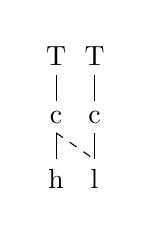
\begin{tikzpicture}[baseline = (m-2-1.base)]
\matrix (m) [matrix of nodes, row sep = 1em]{
T & T \\
c & c \\
h & l \\
};
\draw (m-1-1.south) -- (m-2-1.north);
\draw (m-1-2.south) -- (m-2-2.north);
\draw (m-2-1.south) -- (m-3-1.north);
\draw (m-2-2.south) -- (m-3-2.north);
\draw [dashed] (m-2-1.south) -- (m-3-2.north);
\end{tikzpicture}
\end{exe}
Also, this is the only sandhi alternation in the whole language, meaning no other patterns to create confounds. \par
There are two questions which are important here. One, what is the full tonal inventory in the language? Looking back at Yan (1981), Gao'an is a seven-tone system:
\begin{exe}
\ex
\begin{tabular}[t]{ll|ll|ll|ll}
Category & Tone & Category & Tone & Category & Tone & Category & Tone \\
\hline
\textit{yinping} & 55 & \textit{shang} & 42 & \textit{yinqu} & 33 & \textit{yinru} & 3 \\
\textit{yangping} & 24 & & & \textit{yangqu} & 11 & \textit{yangru} & 1 \\
\end{tabular}
\end{exe}
The phonetic notation is helpful, but how are we to understand the \emph{phonological} form of these tones? A reasonable set of representations is given below:
\begin{exe}
\ex
\begin{tabular}[t]{lll|lll|lll|lll}
Category & Tone & UR & Category & Tone & UR & Category & Tone & UR & Category & Tone & UR \\
\hline
\textit{yinping} & 55 & H & \textit{shang} & 42 & HL & \textit{yinqu} & 33 & M & \textit{yinru} & 3 & Mq \\
\textit{yangping} & 24 & LH & & & &  \textit{yangqu} & 11 & L & \textit{yangru} & 1 & Lq \\
\end{tabular}
\end{exe}
Using this set of representations, and assuming that 53 is akin to [HM], Chen's rule is thus:
\begin{exe}
\ex
H $\rightarrow$ HM / \underline{\hspace{1em}} M, L, Mq, Lq
\end{exe}
The question that concerns us here is whether there is a case for representing the pattern in this language in terms of the melodic tier and \emph{not} at the syllable level. For Gao'an, there does not seem to be any principled reason to not use syllable level representation to posit a rule H $\rightarrow$ F / \underline{\hspace{1em}} M, L, Mq, Lq. One may argue that melody representation clarifies the assimilatory nature of the rule, but this is not necessarily the case; how do we get HM as assimilation before L and Lq, for example? We know that L is `lower' than H, and that the assimilation is one of lowering, but this is not encoded anywhere in the phonology.  \par
We are also faced with the issue of what happens when we devise a rule for the `elsewhere' case:
\begin{exe}
\ex
H $\rightarrow$ H / \underline{\hspace{1em}} H, HL, LH
\end{exe}
This leaves us with the same problem as the Nanjing data. LH is an environment for the elsewhere rule, L is an environment for the lowering rule. But L is a submelody of LH. We could introduce word boundaries such that L\# is the environment, but this won't scale up to strings of more than two syllables (for example, how do we distinguish H.LH (no sandhi predicted) from H.L.H (sandhi is predicted) using only the melody?). Syllable-level representation, on the other hand, avoids this problem, since L and LH are distinct (as L and R). \par
There is suspicion as to whether this process is assimilatory at all. Yan's (1981) data comes from a speaker of the Laowu Zhoujia variety of Gao'an spoken at the Yangxu Commune, approximately 20 km southwest of the county-level city Gao'an. He notes that the two dialects are identical save for some differences in consonant inventories. The \textit{yinping} tone in the Gao'an spoken in the city is pronounced [35] (instead of [55]) with no sandhi alternations reported. If this were indeed a case of assimilation on the melody, we might expect [35] (MH) to become [33] (M), but it doesn't. While this is somewhat speculative, it does raise concerns about how to characterize this process.\par  
What we have shown here is that a case for which sandhi is argued to be operating on the melodic tier (and not at the syllable level) does not hold up to representation in terms of tonal elements in the melody.  
\printbibliography
\end{document}